%\documentclass[slidestop,mathserif]{beamer}
\documentclass[usenames,dvipsnames]{beamer}
%\documentclass{beamer}
%\definecolor{SKIcolor}{rgb}{221,54,49}
%\usecolortheme[named=SKIcolor]{structure}
%\usepackage{beamerthemePostech}
%\usetheme{AnnArbor}
\usetheme{Madrid}
\usepackage{arev}
\usepackage{xcolor}
\usepackage{color}
%\usepackage{subfigure}
\usepackage{multirow}
\usepackage{amsmath}
\usepackage{amsthm}
\usepackage{amsfonts}
\usepackage{hyperref}
\usepackage{mathrsfs}
\usepackage[listings,theorems]{tcolorbox}
\usepackage{algorithm2e}
\usepackage{algpseudocode}
\usepackage{mathtools}
\usepackage{adjustbox}
\usepackage{chngcntr}
\usepackage{kotex}
\usepackage{booktabs}
\usepackage{subfig}
\usepackage{makecell}
\usepackage{forest}
\usepackage[flushleft]{threeparttable}
\def\nine{\fontsize{9pt}{9pt}\selectfont}
\def\eight{\fontsize{8pt}{8pt}\selectfont}
\def\seven{\fontsize{7pt}{7pt}\selectfont}
\def\ttiny{\fontsize{6pt}{6pt}\selectfont}
\def\Tiny{\fontsize{5pt}{5pt}\selectfont}

\addtobeamertemplate{navigation symbols}{}{ \hspace{1em}    \usebeamerfont{footline}%
	\insertframenumber / \inserttotalframenumber }

%% Package, Library, abbreviate terms
\newcommand{\siplibtwo}{\textsf{SIPLIB 2.0}}
\newcommand{\siplib}{\textsf{SIPLIB}}
\newcommand{\miplib}{\textsf{MIPLIB 2010}}
\newcommand{\smps}{\textsf{SMPS}}
\newcommand{\mps}{\textsf{MPS}}
\newcommand{\mpsx}{\textsf{MPSX}}
\newcommand{\jump}{\textsf{JuMP}}
\newcommand{\structjump}{\textsf{StructJuMP}}

% Problems
\newcommand{\airlift}{\textsf{AIRLIFT}}
\newcommand{\chem}{\textsf{CHEM}}
\newcommand{\dcap}{\textsf{DCAP}}
\newcommand{\sdcp}{\textsf{SDCP}}
\newcommand{\mptsps}{\textsf{MPTSPs}}
\newcommand{\sizes}{\textsf{SIZES}}
\newcommand{\smkp}{\textsf{SMKP}}
\newcommand{\sslp}{\textsf{SSLP}}
\newcommand{\suc}{\textsf{SUC}}
\newcommand{\cargo}{\textsf{CARGO}}
\newcommand{\phone}{\textsf{PHONE}}

% Solvers
\newcommand{\dsp}{\textsf{DSP}}
\newcommand{\pysp}{\textsf{PySP}}
\newcommand{\pyomo}{\textsf{Pyomo}}
\newcommand{\cplex}{\textsf{CPLEX}}
\newcommand{\scip}{\textsf{SCIP}}
\newcommand{\pipssbb}{\textsf{PIPS-SBB}}

%% Programming languages
\newcommand{\julia}{\texttt{Julia}}
\newcommand{\python}{\texttt{Python}}
\newcommand{\clang}{\texttt{C}}
\newcommand{\cpp}{\texttt{C++}}
\newcommand{\matlab}{\texttt{MATLAB}}

%% Siplib.jl related terms
\newcommand{\jumpmodel}{\texttt{JuMP.Model}}
\newcommand{\siplibjl}{\texttt{Siplib.jl}}

\setcounter{tocdepth}{2}

% for Siplib.jl tree
\definecolor{folderbg}{RGB}{124,166,198}
\definecolor{folderborder}{RGB}{110,144,169}
\def\Size{4pt}
\tikzset{
	folder/.pic={
		\filldraw[draw=folderborder,top color=folderbg!50,bottom color=folderbg]
		(-1.05*\Size,0.2\Size+5pt) rectangle ++(.75*\Size,-0.2\Size-5pt);  
		\filldraw[draw=folderborder,top color=folderbg!50,bottom color=folderbg]
		(-1.15*\Size,-\Size) rectangle (1.15*\Size,\Size);
	}
}

% for Julia script
\lstdefinelanguage{julia}
{
	sensitive=true,	
	basicstyle=\ttfamily\scriptsize,
	columns=fullflexible, % make sure to use fixed-width font, CM typewriter is NOT fixed width
	numbers=left, 
	numberstyle=\small\ttfamily\color{Gray},
	stepnumber=0,              
	numbersep=10pt, 
	numberfirstline=true, 
	numberblanklines=true, 
	tabsize=4,
	lineskip=-1.5pt,
	extendedchars=true,
	breaklines=true,        
	keywordstyle=\color{Blue}\bfseries,
	identifierstyle=, % using emph or index keywords
	commentstyle=\sffamily\color{OliveGreen},
	stringstyle=\color{Maroon},
	showstringspaces=false,
	showtabs=false,
	upquote=false,
	keywordsprefix=\@,
	keywords={exit,whos,edit,load,is,isa,isequal,typeof,tuple,ntuple,uid,hash,finalizer,convert,promote,
		subtype,typemin,typemax,realmin,realmax,sizeof,eps,promote_type,method_exists,applicable,
		invoke,dlopen,dlsym,system,error,throw,assert,new,Inf,Nan,pi,im,begin,while,for,in,return,
		break,continue,macro,quote,let,if,elseif,else,try,catch,end,bitstype,ccall,do,using,module,
		import,export,importall,baremodule,immutable,local,global,const,Bool,Int,Int8,Int16,Int32,
		Int64,Uint,Uint8,Uint16,Uint32,Uint64,Float32,Float64,Complex64,Complex128,String,Symbol,Any,Nothing,None,
		function,type,typealias,abstract,struct, mutable},
	comment=[l]{\#},
	%morecomment=[s]{#=}{=#},
	morestring=[d]\',
	morestring=[b]\",
}

%\newtheorem{lemma}{Lemma}
\newtheorem{proposition}{Proposition}
\newcommand{\argmin}{\arg\!\min}
\newcommand{\argmax}{\arg\!\max}
\DeclarePairedDelimiter{\ceil}{\lceil}{\rceil}
\DeclarePairedDelimiter{\floor}{\lfloor}{\rfloor}
\DeclareMathOperator*{\PP}{\mathbb{P}}
\DeclareMathOperator*{\EE}{\mathbb{E}}
\SetKwRepeat{Do}{do}{while}    
\setlength\abovecaptionskip{-3pt}
\setbeamertemplate{footline}[frame number]
\counterwithin*{equation}{section}      %식번호를 섹션이 바뀔때마다 초기화하라 \usepackage{chngcntr} 필요
\counterwithin*{equation}{subsection}

% enumerate 번호 기억
\newcounter{savedenum}
\newcommand*{\saveenum}{\setcounter{savedenum}{\theenumi}}
\newcommand*{\resume}{\setcounter{enumi}{\thesavedenum}}

%\setbeamercovered{transparent}
\setbeamercovered{invisible}

%\fboxsep=10mm%padding thickness
\fboxrule=0.7pt%border thickness

% Contents에 한글 표시
\hypersetup{
	unicode=true, %
}
\title{\textbf{SIPLIB 2.0}}
\subtitle{Stochastic Integer Programming Library version 2}

\author{\underline{Yongkyu Cho}\inst{1}\inst{2} \and Kibaek Kim\inst{2} \\ \and James Luedtke\inst{3} \and Jeffrey Linderoth\inst{3}}
\institute[] % (optional, but mostly needed)
{
	\inst{1}%
	Department of Industrial and Management Engineering\\
	Pohang University of Science and Technology
	\and
	\inst{2}%
	Mathematics and Computer Science Division\\
	Argonne National Laboratory
	\and
	\inst{3}%
	Department of Industrial and Systems Engineering\\
	University of Wisconsin-Madison
}
\date{INFORMS Annual Meeting 2018}


\begin{document}
	
	\tcbset{%
		noparskip,
		colback=white, %background color of the box
		colframe=black, %color of frame and title background
		coltext=black, %color of body text
		coltitle=white, %color of title text 
		fonttitle=\bfseries,
	}
	
	\setbeamercovered{transparent=30}
	\begin{frame}
	\titlepage
\end{frame}

\frame{
	\frametitle{Contents}
	\tableofcontents[hideothersubsections]
	\setcounter{tocdepth}{2}
}

\section{Overview}
\begin{frame}<beamer>{Contents}
\tableofcontents[currentsection,currentsubsection,hideothersubsections]
\end{frame}	

\begin{frame}{What is \siplib?}
\footnote{\tiny Available at: \href{https://www2.isye.gatech.edu/~sahmed/siplib/}{https://www2.isye.gatech.edu/~sahmed/siplib/}}{\siplib}: A Stochastic Integer Programming Test Problem Library
\begin{itemize}
\item \siplib\ is a collection of test problems to facilitate \textcolor{blue}{computational and algorithmic research} in stochastic integer programming (SIP).
\item The test problem data is provided in the \textcolor{blue}{standard format (\smps)} unless otherwise mentioned.
\item Where available, \textcolor{blue}{information on the underlying problem formulation} and \textcolor{blue}{known solution} is also included.
\end{itemize}
\end{frame}

\begin{frame}{Limitation of the former \siplib}
\pause
\begin{enumerate}
\invisible<-1>{\item Number of the instances}
\begin{itemize}
\invisible<-1>{\item Researchers in this field need more test set.}
\end{itemize}
\pause
\invisible<-2>{\item Variation of problem types}
\begin{itemize}
\invisible<-2>{\item Provides only 5 different variations in terms of three variable types: continuous, binary, integer.}
\end{itemize}
\pause
\invisible<-3>{\item Contribution rule}
\begin{itemize}
\invisible<-3>{\item Different problem provides different information.}
\invisible<-3>{\item For some problems, only limited information is available.}
\end{itemize}
\end{enumerate}
\end{frame}

\begin{frame}{Contribution of \siplibtwo}
\textbf{\siplibtwo\ provides}
\pause
\begin{itemize}
\invisible<-1>{\item \textcolor{blue}{more instances} accompanied with analytic \& computational information}
\pause
\invisible<-2>{\item \textcolor{blue}{a \julia\ package} to support}
\begin{itemize}
\invisible<-2>{\item \textcolor{blue}{generating new instances in SMPS format}}
\invisible<-2>{\item analyzing the instances (size, sparsity)}
\invisible<-2>{\item solving the instances to get some known bounds}
\end{itemize}
\pause
\invisible<-3>{\item \textcolor{blue}{all the details} about the problems}
\begin{itemize}
\invisible<-3>{\item formulation, deterministic \& random parameters}
\invisible<-3>{\item parameterized modeling scripts written in \julia\ language}
\end{itemize}
\end{itemize}
\end{frame}

\section{Stochastic Integer Programming}

\begin{frame}<beamer>{Contents}
\tableofcontents[currentsection,currentsubsection,hideothersubsections]
\end{frame}

\begin{frame}{Problem of interest}
\textbf{{Two-stage Stochastic Integer Programming (TSSIP)}}
\pause
\begin{itemize}
\invisible<-1>{\item Considers only \textcolor{blue}{two stages}.}
\begin{itemize}
\invisible<-1>{\item \textcolor{blue}{Present} (first-stage) and \textcolor{blue}{Future} (second-stage)}
\end{itemize}
\pause 
\invisible<-2>{\item First-stage decision must be made \textcolor{blue}{for now}.}
\invisible<-2>{\item Second-stage decision can be made \textcolor{blue}{after the future is realized} (called \textit{recourse} action).}
\pause
\invisible<-3>{\item First-stage decision can affect the second-stage decision.}
\end{itemize}
\end{frame}

\begin{frame}[shrink=15]{Mathematical formulation}
\textbf{TSSIP:}
\begin{align}
\min_{x\in X}{\left\{c^\top x + \textcolor{blue}{\mathcal{Q}(x)}:\ Ax\ge b\right\}} \label{eq:SIP_1}
\end{align}
\vspace{-0.4cm}
\begin{itemize}
\item $X\subseteq \mathbb{R}^{n_1-k_1}\times\mathbb{Z}^{k_1}$
\item $c\in\mathbb{R}^{n_1}$
\item $A\in\mathbb{R}^{m_1\times n_1}$
\item $b\in\mathbb{R}^{m_1}$
\item \textcolor{blue}{$\mathcal{Q}(x):=\EE_{\pmb{\xi}}[Q(x,\pmb{\xi})]$ (expected recourse function)}
\item $\pmb{\xi}$ is a random element defined on a probability triple $(\Xi, \mathcal{F},\PP)$
\end{itemize}
\vspace{0.4cm}
\textbf{\textcolor{blue}{Recourse function}} \textcolor{blue}{$Q(\cdot,\cdot)$}:
\begin{align}
\textcolor{blue}{Q(x,\xi_s):=\min_{y\in Y}\left\{q(\xi_s)^\top y : W(\xi_s)y\ge h(\xi_s)-T(\xi_s)x\right\}}
\end{align}
\vspace{-0.4cm}
\begin{itemize}
\item $\xi_s$ is a realized random element (called \textit{scenario})
\item $Y\subseteq\mathbb{R}^{n_2-k_2}\times\mathbb{Z}^{k_2}$
\item $q(\xi_s)\in\mathbb{R}^{n_2}$
\item $W(\xi_s)\in\mathbb{R}^{m_2\times n_2}$
\item $h(\xi_s)\in\mathbb{R}^{m_2}$
\item $T(\xi_s)\in\mathbb{R}^{m_2\times n_1}$
\end{itemize}		
\end{frame}

\begin{frame}{Mathematical formulation}
\textbf{Extensive Form} (EF):
\begin{subequations}\label{sip:ef}
\begin{align}
\min_{x,\mathrm{y}}\ &c^{\top}x + \sum_{s=1}^{r}\PP(s) (q_s^{\top}y_s) \label{ef:obj}\\ 
\mathrm{s.t.}\ &Ax\ge b,  \label{ef:b}\\
&T_s x+W_s y_s\ge h_s,\quad\forall s\in\{1,\ldots,r\}, \label{ef:c} \\
&x\in X, \label{ef:d} \\
&y_s \in Y,\quad\forall s\in\{1,\ldots,r\}. \label{ef:e}
\end{align}
\end{subequations}
\vspace{-0.4cm}
\begin{itemize}
\item $\mathrm{y}:=\{y_1,y_2,\ldots,y_r\}$
\item $q_s:=q(\xi_s)$
\item $W_s:=W(\xi_s)$
\item $h_s:=h(\xi_s)$
\item $T_s:=T(\xi_s)$
\end{itemize}
\end{frame}

\begin{frame}{EF: Block-diagonal structure}
\begin{figure}
\begin{center}
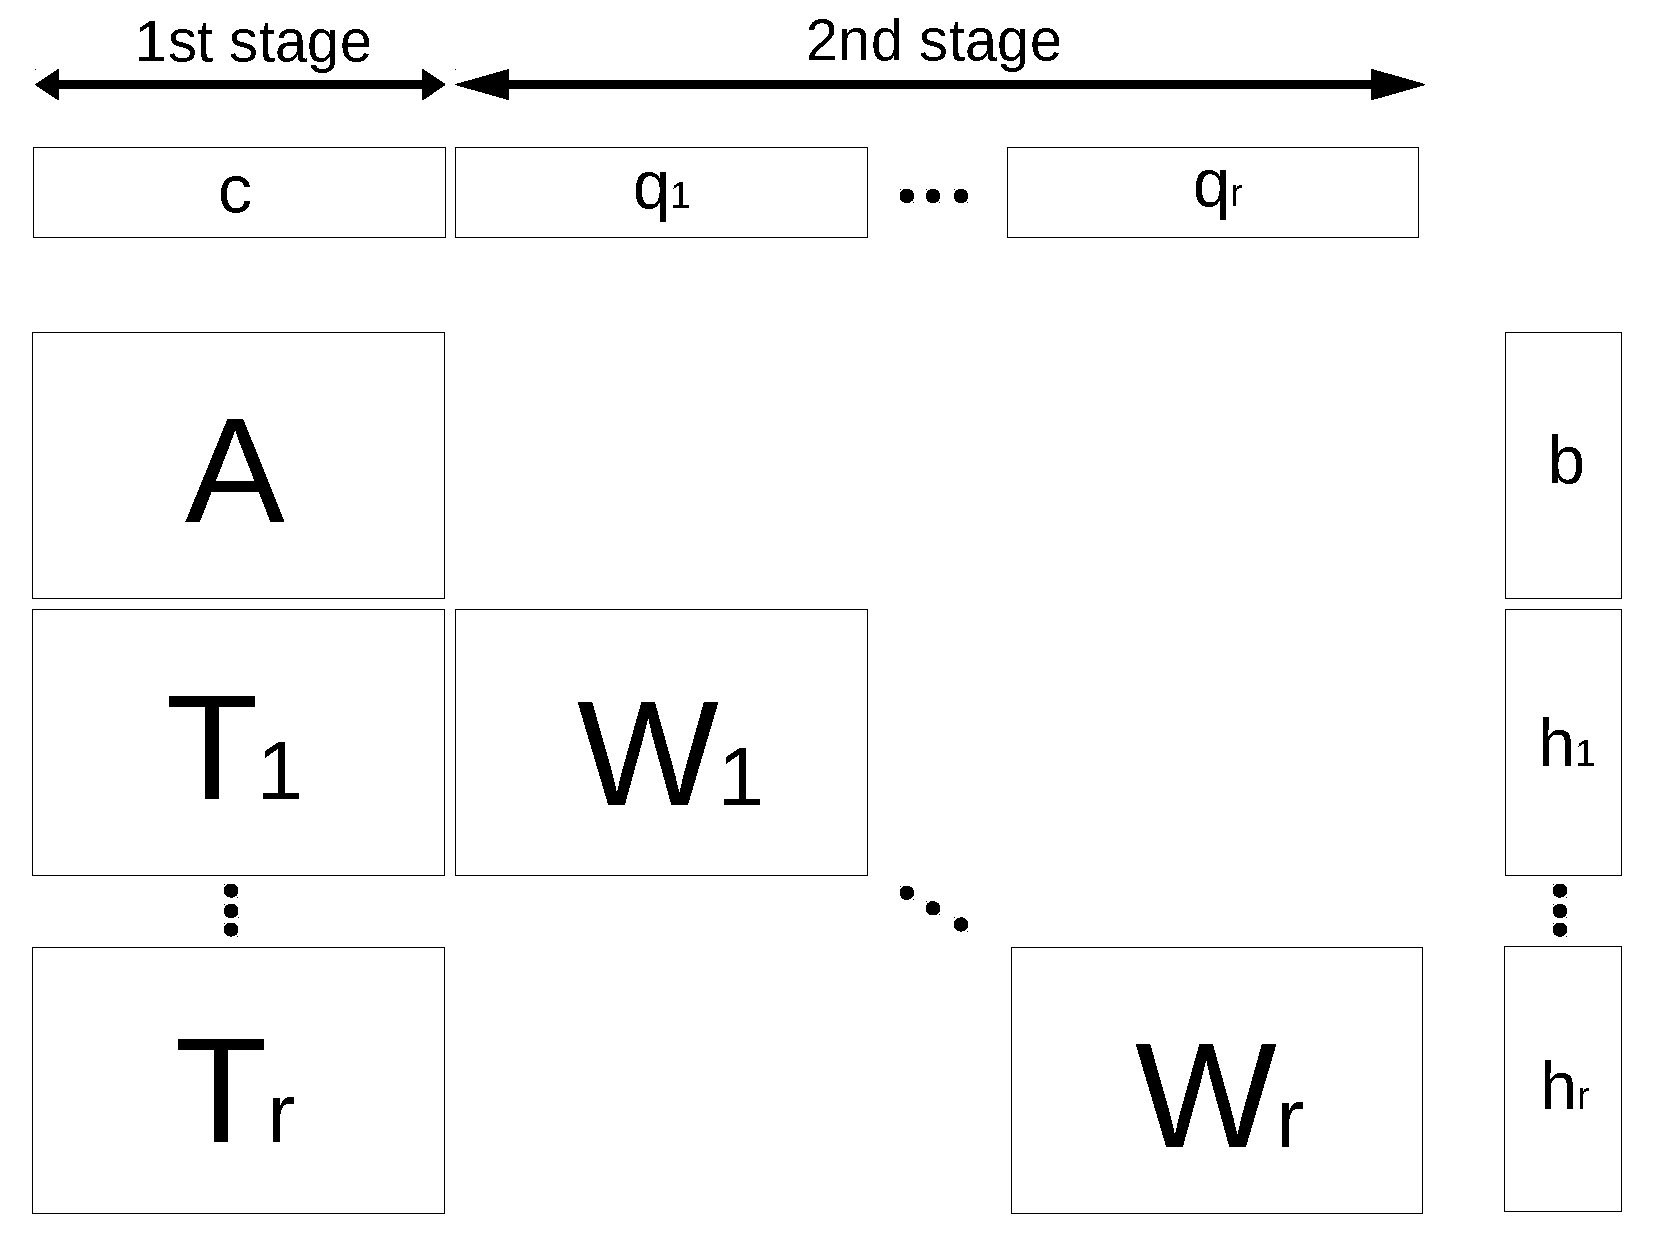
\includegraphics[width=0.9\textwidth]{stagewise_sparsity_slide}
\end{center}
\end{figure}
\end{frame}

\begin{frame}{EF: Block-diagonal structure}
\vspace{-0.5cm}
\begin{figure}
\centering
\subfloat[][AIRLIFT\_3]
{
\centering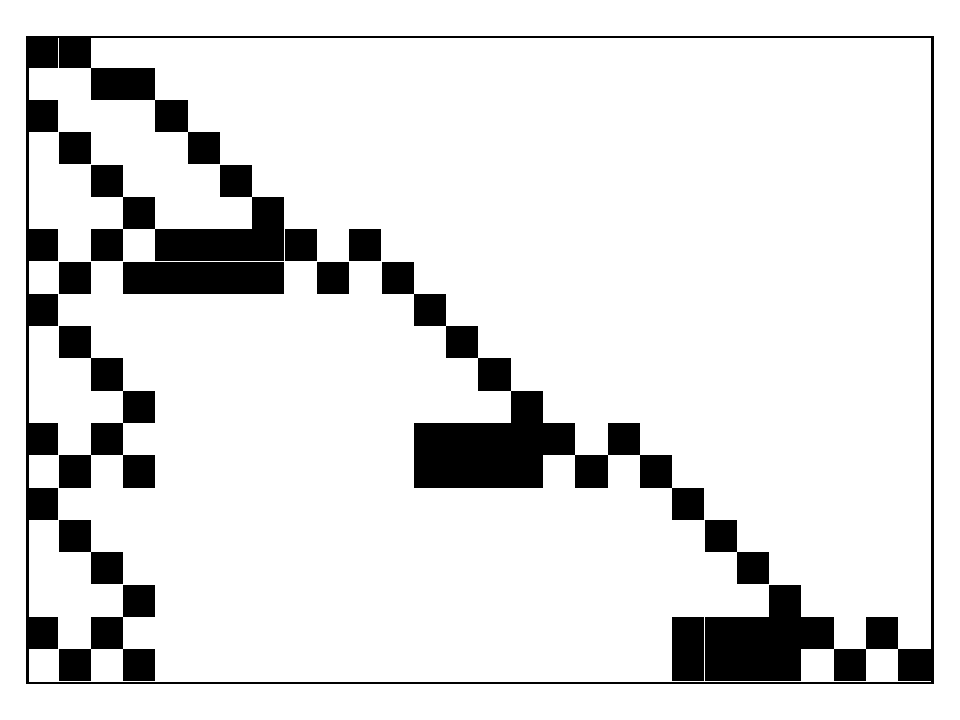
\includegraphics[width=0.35\linewidth]{AIRLIFT_3}
}
~
\subfloat[][CHEM\_3]
{
\centering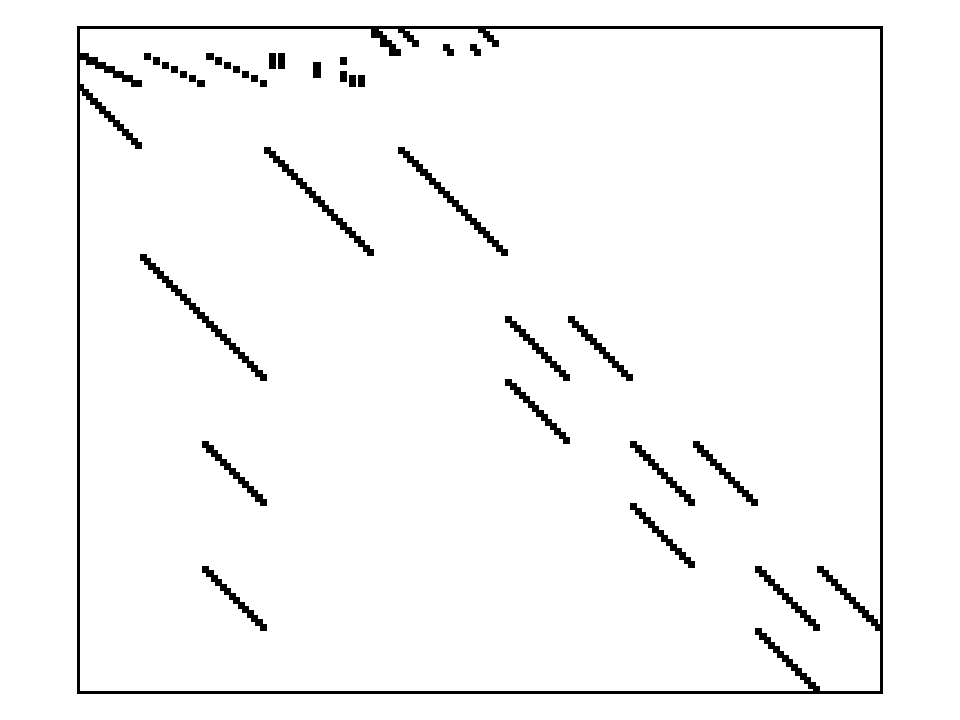
\includegraphics[width=0.35\linewidth]{CHEM_3}
}
\vspace{-0.05cm}
\subfloat[][DCAP\_3\_3\_3\_3]
{
\centering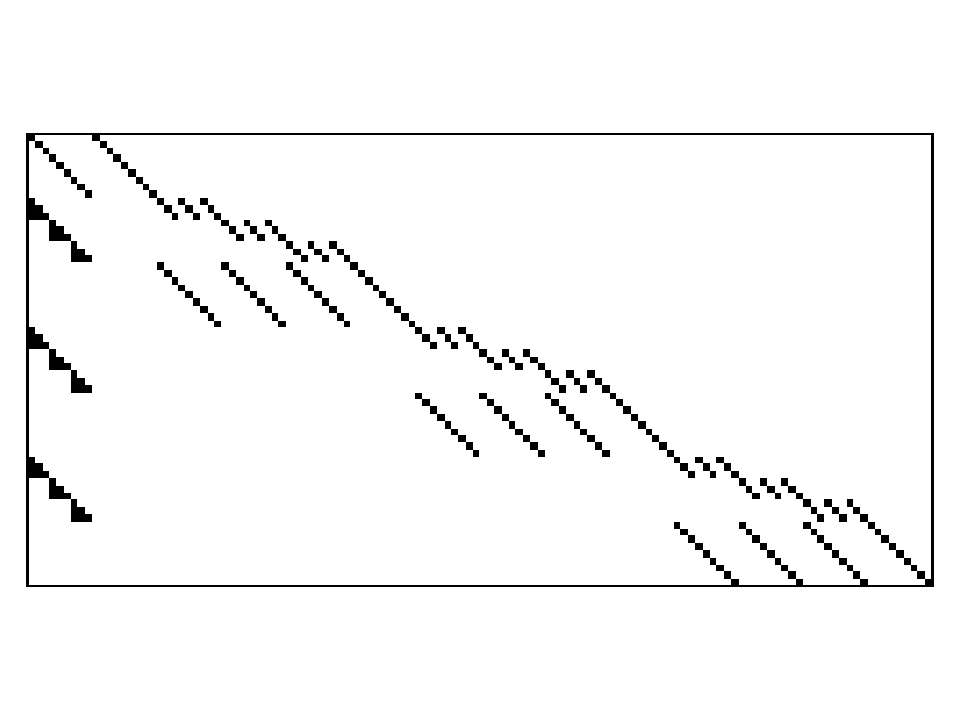
\includegraphics[width=0.35\linewidth]{DCAP_3_3_3_3}
}
~
\subfloat[][SSLP\_5\_10\_3]
{
\centering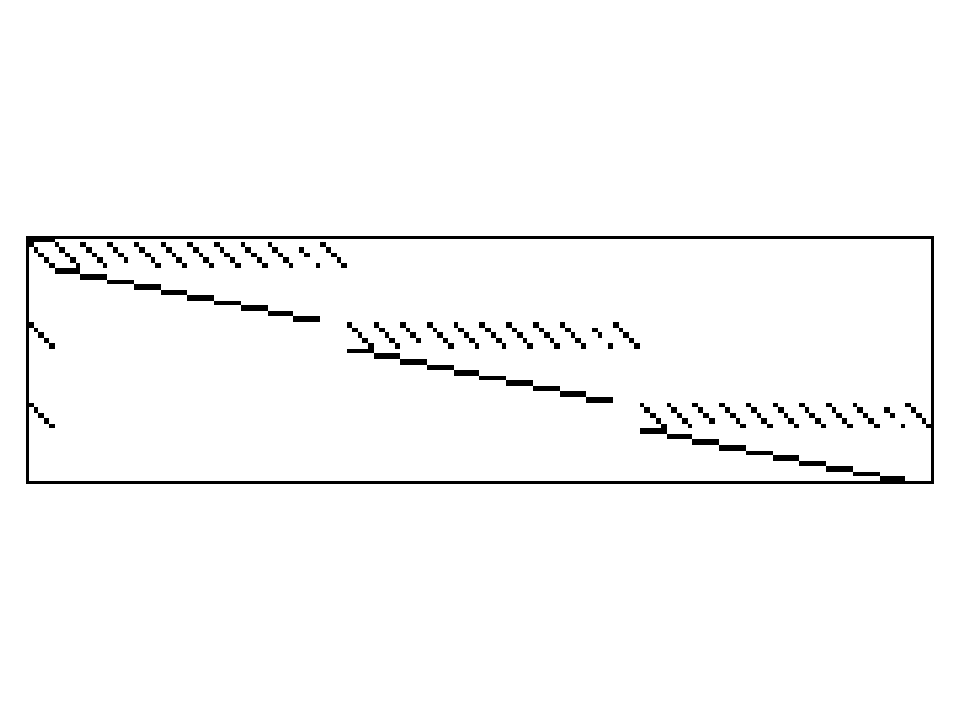
\includegraphics[width=0.35\linewidth]{SSLP_5_10_3}
}
\vspace{0.5cm}
\caption{Example: Repeated sparsity patterns in EF}
%\label{data3}
\end{figure}
\end{frame}

\section{Main tools: SMPS and StructJuMP}
\begin{frame}<beamer>{Contents}
\tableofcontents[currentsection,currentsubsection,hideothersubsections]
\end{frame}	

\begin{frame}{\texttt{SMPS} format}
\textbf{\footnote{\tiny For details: \href{http://plato.asu.edu/ftp/smps.pdf}{http://plato.asu.edu/ftp/smps.pdf}}{\smps} is a \textcolor{blue}{standard column-oriented data format} for stochastic programs.} 
\begin{itemize}
\item \textbf{(example)} Let DCAP\_3\_3\_3\_10 be the instance name. Then, \smps\ format comprises
\begin{itemize}
\item DCAP\_3\_3\_3\_10.cor
\item DCAP\_3\_3\_3\_10.tim
\item DCAP\_3\_3\_3\_10.sto
\end{itemize}
\item The role of each file
\begin{itemize}
\item \textbf{\texttt{.cor}}: Core file written in \mps\ format. This describes the \textcolor{blue}{fundamental problem structure.}
\item \textbf{\texttt{.tim}}: Time file which specifies \textcolor{blue}{the location where each stage begins.}
\item \textbf{\texttt{.sto}}: Stoch file which contains \textcolor{blue}{scenario data.}
\end{itemize}
\end{itemize}
\end{frame}

\begin{frame}{\texttt{SMPS} format: Graphical description}
\vspace{-0.35cm}
\begin{figure}
\begin{center}
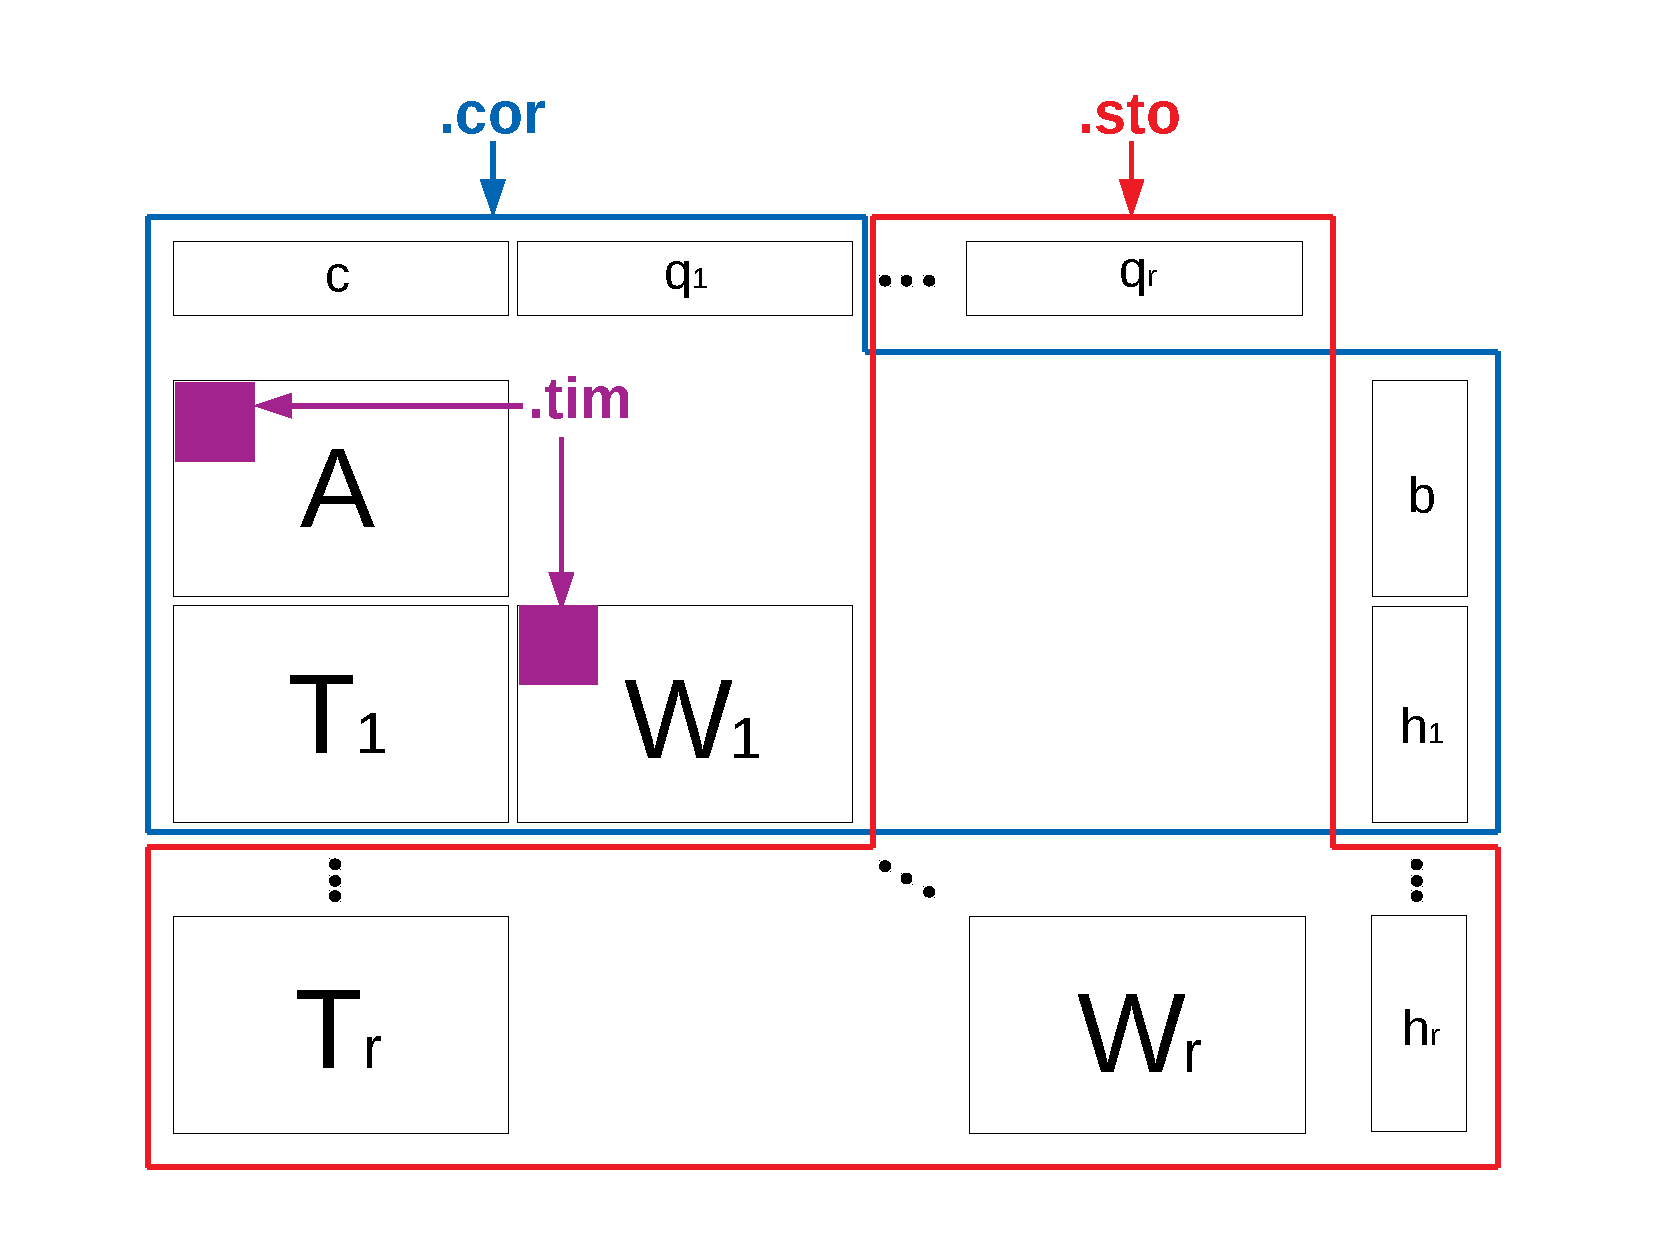
\includegraphics[width=\textwidth]{SMPS_description_slide}
\end{center}
\end{figure}
\end{frame}
%
%\begin{frame}{\julia\ language}
%\textbf{\footnote{\tiny Available at: \href{https://julialang.org /}{https://julialang.org/}}{Julia programming language} is a \textcolor{blue}{flexible dynamic language}, appropriate for \textcolor{blue}{scientific and numerical computing}, with \textcolor{blue}{performance} comparable to traditional statically-typed languages.} 
%\begin{figure}
%\begin{center}
%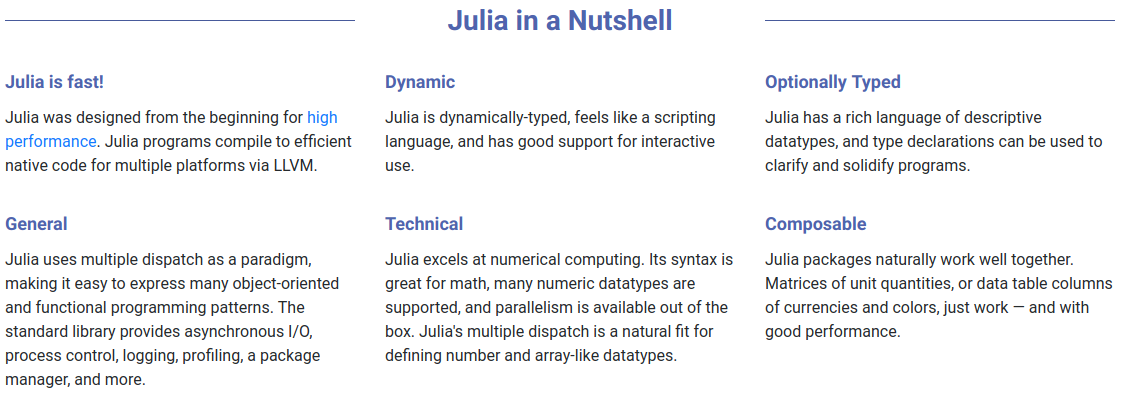
\includegraphics[width=\textwidth]{julia_nutshell}
%\end{center}
%\end{figure}	
%\end{frame}

\begin{frame}{\structjump\ package}
\textbf{\footnote{\tiny Available at: \href{https://github.com/StructJuMP/StructJuMP.jl}{https://github.com/StructJuMP/StructJuMP.jl}}{\structjump} is a \julia\ package for modeling structured optimization models.}
\begin{itemize}
\item \textbf{\structjump} is an \textcolor{blue}{extension of \textbf{\jump} package}, a domain-specific modeling language for mathematical optimization embedded in \julia.
\begin{itemize}
\item \textbf{\jump} is generic, fast, and straightforward modeler.
\end{itemize}
%\item \textbf{\structjump} provides a parallel algebraic modeling framework for \textcolor{blue}{block-structured optimization models} in \julia.
\item \textbf{\structjump} constructs a \textcolor{blue}{\textbf{\jumpmodel}-type object} that contains every information of an SIP instance.
\end{itemize}
\end{frame}

\begin{frame}[shrink=40]{Example: Modeling \dcap\ with \structjump}
%\underline{\emph{\textbf{DCAP: Extensive Form}}}
\begin{columns}
	\begin{column}{10cm}
	%	\begin{tcolorbox}[title=MIP$_O$]
			\vspace{-0.5cm}
			\begin{flushleft}
%				\begin{subequations*} \label{dcap:formulation}
					\begin{align*}
					\textrm{min}\ &\sum_{t\in T}\sum_{i\in R}\left(\alpha_{it}x_{it}+\beta_{it}u_{it}\right)+\sum_{s\in\mathcal{S}}\PP(s)\sum_{t\in T}\sum_{i\in R\cup\{0\}}\sum_{j\in N}c_{ijt}^{s}y_{ijt}^s	 \\
					\textrm{s.t.}\ & x_{it}\le \textrm{M}u_{it},\quad\forall i\in R,\ \forall t\in T,\\
					&\sum_{j\in N}d_{jt}^s y_{ijt}^s\le\sum_{\tau=1}^{t}x_{i\tau},\quad\forall i\in R,\ \forall t\in T,\ \forall s\in\mathcal{S},\\
					&\sum_{i\in R\cup \{0\}}y_{ijt}^s=1,\quad\forall j\in N,\ \forall t\in T,\ \forall s\in\mathcal{S},  \\
					&x_{it}\ge 0,\quad\forall i\in R,\ \forall t\in T, \\
					&u_{it}\in\{0,1\}, \quad\forall i\in R,\ \forall t\in T,\\
					&y_{ijt}^s\in\{0,1\},\quad\forall i\in R\cup\{0\},\ \forall j\in N,\ \forall t\in T,\ \forall s\in\mathcal{S}.
					\end{align*}
%				\end{subequations*}
			\end{flushleft}
			\vspace{0.5cm}
			\centering \textcolor{Blue}{Formulation:} \dcap\ (extensive form)
%		\end{tcolorbox}
	\end{column}
	
	\begin{column}{10cm}
		\vspace{1cm}
		\begin{figure}
			\centering
			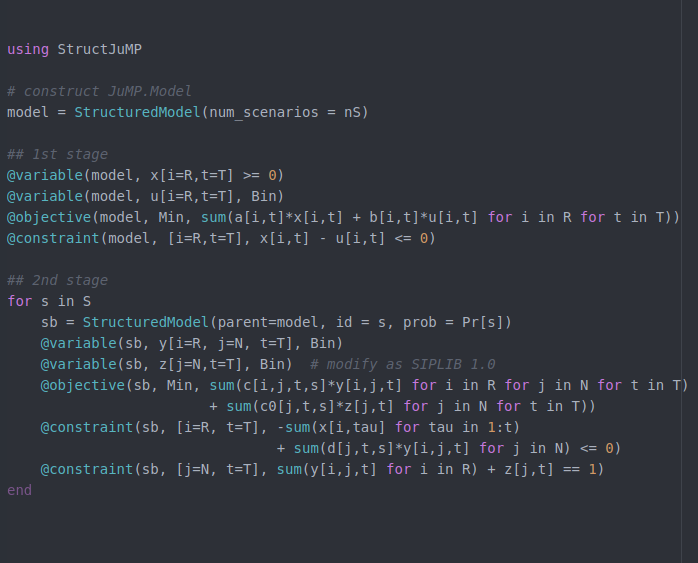
\includegraphics[width=\textwidth,keepaspectratio]{dcap_structjump}
			\vspace{0.3cm}
			\caption{\dcap\ (modeling script using \structjump)}
		\end{figure}
	\end{column}
\end{columns}
\end{frame}



\section{Implementation of a Julia Package: Siplib.jl}
\begin{frame}<beamer>{Contents}
\tableofcontents[currentsection,currentsubsection,hideothersubsections]
\end{frame}	

\begin{frame}{Core functionality of \siplibjl}
\textbf{Generating \smps\ files of SIP instance}:
\pause
\begin{figure}
\begin{center}
\invisible<-1>{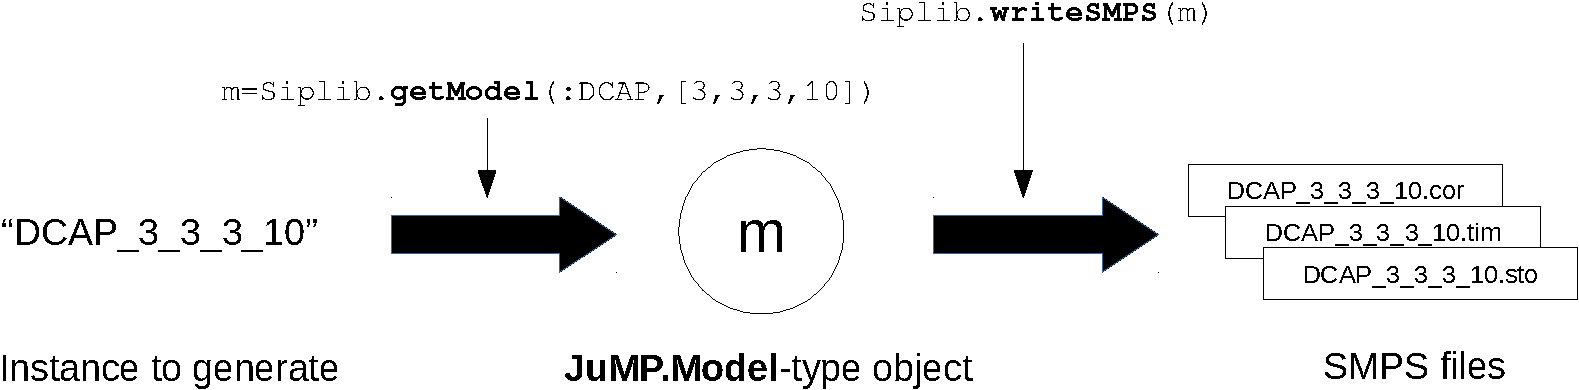
\includegraphics[width=\textwidth]{siplib_package}}
\end{center}
\end{figure}	
\end{frame}

\begin{frame}{Problems available in \siplibtwo}
We implement \texttt{Julia} scripts for modeling \textcolor{blue}{11 different problems} from various sources and embed them into \siplibjl.
\ttiny
		\begin{table}[H]
	\centering
	%\resizebox{}{!}{%
	\label{table:problems}
	\begin{tabular}{@{}llll@{}}
		\toprule
		\textbf{Problem}		  		  & Description                                                        & Main reference              \\ \midrule
		\textbf{\airlift} & Airlift operations scheduling & Midler and Wollmer (1969)  \\
		\textbf{\cargo} & Cargo network scheduling  & Mulvey and Ruszczy\`{n}ski (1995) \\
		\textbf{\chem} & Design of batch chemical plants& Subrahmanyam et al. (1994) \\				
		\textbf{\dcap}         & \makecell[tl]{Dynamic capacity planning with stochastic\\ demand  }                  & Ahmed and Garcia (2003)                           \\
		\textbf{\mptsps}       & \makecell[tl]{Multi-path traveling salesman problem with\\ stochastic travel costs } & Tadei et al. (2017)                             \\
		\textbf{\phone}       & Telecommunication network planning & Sen et al. (2004)                            \\
		\textbf{\sdcp} 	& Stochastic data center placement  & Kim et al. (2017) \\
		\textbf{\sizes}        & \makecell[tl]{Optimal product substitution with stochastic\\ demand}         & Jorjani et al. (1999)        \\
		\textbf{\smkp}		  & Stochastic multiple knapsack problem                               & Angulo et al. (2016)                           \\
		\textbf{\sslp}         & Stochastic server location problem                                 & Ntaimo and Sen (2005)                           \\
		\textbf{\suc}         & Stochastic unit commitment problem			               & Papavasiliou and Oren (2013)                        \\ \bottomrule
	\end{tabular}%
\end{table}
\end{frame}

\begin{frame}{Problems available in \siplibtwo}
We \textcolor{blue}{parameterize the problems} to let users tailor the instances and generate \smps\ files as they want.
\ttiny
		\begin{table}[H]
	\centering
	%			\caption{Instance naming rules}
	\label{table:naming_rule}
	\resizebox{\textwidth}{!}{%
		\begin{tabular}{@{}llp{0.6\textwidth}}
			%		\begin{tabular}{@{}llp{3in}}
			\toprule
			Problem & \textbf{Instance name}                 & \multicolumn{1}{c}{Remark}                                                                    					      \\ \midrule
			\airlift	& \textbf{AIRLIFT\_$\mathcal{S}$}& $\mathcal{S}$: number of scenarios\\
			\cargo	& \textbf{CARGO\_$\mathcal{S}$}& $\mathcal{S}$: number of scenarios\\		
			\chem	& \textbf{CHEM\_$\mathcal{S}$}& $\mathcal{S}$: number of scenarios\\				
			\dcap\    & \textbf{DCAP\_$R$\_$N$\_$T$\_$\mathcal{S}$}    &   $R$: number of resources, $N$: number of tasks, $T$: number of time periods, $\mathcal{S}$: number of scenarios        \\
			\mptsps\  & \textbf{MPTSPs\_$d$\_$N$\_$\mathcal{S}$} &$d$: node distribution strategy, $N$: number of nodes, $\mathcal{S}$: number of scenarios\\
			\phone	& \textbf{PHONE\_$\mathcal{S}$}& $\mathcal{S}$: number of scenarios\\
			\sdcp\ & \textbf{SDCP\_$k$\_$p$\_$d$\_$\mathcal{S}$} & $k$: maximum number of dispatchable loads, $p$: wind penetration level (\%), $d$: day type, $\mathcal{S}$: number of scenarios\\
			\sizes\   & \textbf{SIZES\_$\mathcal{S}$}                            & $\mathcal{S}$: number of scenarios   															\\
			\smkp\    &   \textbf{SMKP\_$I$\_$\mathcal{S}$}    &   $I$: number of types for item, $\mathcal{S}$: number of scenarios  													 \\
			\sslp\    &  \textbf{SSLP\_$I$\_$J$\_$\mathcal{S}$}      &    $I$: number of clients, $J$: number of server locations, $\mathcal{S}$: number of scenarios                 				   \\
			\suc\    & 	\textbf{SUC\_$d$\_$\mathcal{S}$}    &  $d$: day type, $\mathcal{S}$: number of scenarios                                                 						 \\ \bottomrule
		\end{tabular}%
	}
\end{table}
\end{frame}

\begin{frame}{Components of the problems}
We classify the problems based on their \textcolor{blue}{stage-wise variable types.}		
\begin{table}[H]
\seven
\centering
%			\caption{Components of the problems}
\label{table:prob_class}
\begin{threeparttable}
\begin{tabular}{@{}lllll@{}}
\toprule
& \multicolumn{2}{c}{1st stage}                              				  	& \multicolumn{2}{c}{2nd stage}                             			        \\ \midrule
Problem 	     & Variable                    & Constraint                   	& Variable                    & Constraint                  				    \\ \midrule
\airlift\  & $\mathbb{I}$ & \texttt{IKN}& $\mathbb{C}$, $\mathbb{I}$ & \texttt{BIN}, \texttt{GEN}\\
\cargo\  & $\mathbb{I}$ & \texttt{IKN} & $\mathbb{C}$ & \texttt{GEN}\\		
\chem\  & $\mathbb{C}$, $\mathbb{I}$ & \texttt{VBD}, \texttt{GEN} & $\mathbb{C}$, $\mathbb{B}$ & \texttt{GEN}\\				
\dcap\     & $\mathbb{C}$, $\mathbb{B}$  & \texttt{VBD}                	& $\mathbb{B}$                & \texttt{PAR}, \texttt{M01} 			    		\\
\mptsps\   & $\mathbb{C}$, $\mathbb{B}$  & \texttt{PAR}, \texttt{GEN}		& $\mathbb{B}$                & \texttt{GEN}               						\\
\phone\  & $\mathbb{C}$ & \texttt{IVK} & $\mathbb{C}$, $\mathbb{I}$ & \texttt{GEN} \\			
\sdcp\ & $\mathbb{I}$ & \texttt{IKN}& $\mathbb{C}$ & \texttt{GEN}\\
\sizes\  & $\mathbb{I}$ 			   & \texttt{VBD}, \texttt{GEN} 	& $\mathbb{B}$, $\mathbb{I}$  & \texttt{IKN}             						\\
\smkp\   & $\mathbb{B}$                & \texttt{KNA}                	& $\mathbb{B}$                & \texttt{KNA}              						\\
\sslp\   & $\mathbb{B}$                & \texttt{IVK}, \texttt{GEN} 	& $\mathbb{C}$, $\mathbb{B}$  & \texttt{GEN}             						\\
\suc\   & $\mathbb{C}$, $\mathbb{B}$                 & \texttt{VBD}, \texttt{GEN}       	& $\mathbb{C}$, $\mathbb{B}$  &  \texttt{VBD}, \texttt{GEN}                                  					\\ \bottomrule
\end{tabular}
\end{threeparttable}
\end{table}
\vspace{-0.5cm}
\begin{itemize}
\item $\mathbb{C}$: continuous, $\mathbb{B}$: binary, $\mathbb{I}$: integer
\item We have \textcolor{blue}{10 non-redundant combinations.}
\item Constraint type notation is adopted from \footnote{\tiny Available at: \href{http://miplib.zib.de/miplib2010.php}{http://miplib.zib.de/miplib2010.php}}{\miplib}.
\end{itemize}
\end{frame}

%	\begin{frame}[shrink=45]{Structure of the package}
%		\vspace{1cm}
%		\begin{minipage}[c][1.3\paperheight][c]{\textwidth}
%			\begin{figure} 
%				\begin{forest}
%					for tree={
%						font=\ttfamily,
%						grow'=0,
%						child anchor=west,
%						parent anchor=south,
%						anchor=west,
%						calign=first,
%						inner xsep=7pt,
%						edge path={
%							\noexpand\path [draw, \forestoption{edge}]
%							(!u.south west) +(7.5pt,0) |- (.child anchor) pic {folder} \forestoption{edge label};
%						},
%						% style for your file node 
%						file/.style={edge path={\noexpand\path [draw, \forestoption{edge}]
%								(!u.south west) +(7.5pt,0) |- (.child anchor) \forestoption{edge label};},
%							inner xsep=2pt,font=\small\ttfamily
%						},
%						before typesetting nodes={
%							if n=1
%							{insert before={[,phantom]}}
%							{}
%						},
%						fit=band,
%						before computing xy={l=15pt},
%					}  
%					[Siplib
%					[src
%					[problems
%					[AIRLIFT
%					[DATA
%					[numerical\_data.csv,file]
%					]
%					[AIRLIFT\_model.jl,file]
%					[AIRLIFT\_data.jl,file]
%					]
%					[CARGO
%					[CARGO\_model.jl,file]			
%					]
%					[$\ldots$]
%					]
%					[Siplib.jl,file]
%					[analyzer.jl,file]
%					[generator.jl,file]
%					[writer.jl,file]
%					[solver.jl,file]
%					[utility.jl,file]
%					[problem\_info.csv,file]
%					]
%					]
%					]
%				\end{forest}
%	%			\caption{Structure of the \julia\ package}\label{fig:siplibjl_structure}
%			\end{figure}
%		\end{minipage} 
%	\end{frame}

\section{Computational Experiments (in progress)}
\begin{frame}<beamer>{Contents}
\tableofcontents[currentsection,currentsubsection,hideothersubsections]
\end{frame}	

\begin{frame}{Computing environment}
\begin{figure}
\begin{center}
\includegraphics[width=0.4\textwidth]{Bebop}
\end{center}
\end{figure}
%		\vspace{-1cm}
\begin{table}[H]
\centering
%			\caption{Experimental setting}
\label{table:experimental_setting}
\resizebox{\textwidth}{!}{%
\begin{tabular}{|l|l|}
\hline
\multirow{4}{*}{Computing facility} & \footnote{\tiny 1024-node computing cluster in Argonne National Lab (ANL):  \href{https://www.lcrc.anl.gov/systems/resources/bebop/}{https://www.lcrc.anl.gov/systems/resources/bebop/}}{\textit{Bebop}} with each node      \\
& - CPU: Intel Xeon Processor E5-2695 v4 (36 cores, 36 threads) \\
& - Clock speed: 2.10GHz (maximum 3.30GHz)                     \\
& - Memory:128GB (45MB Smart cache)                            \\ \hline
\multirow{2}{*}{Solver}                & General purpose MIP solver: CPLEX 12.8                                \\
& Open-source Dual Decomposition based SIP solver: DSP                                      \\ \hline
Multi-threading per instance                 & 36                                                           \\ \hline
Time limit per instance                            & 1 hours                                                      \\ \hline
\end{tabular}
}
\end{table}
\end{frame}

\begin{frame}{Computational report (in progress)}
\begin{table}[H]
\centering
\caption{Computational report (tentative)}
\vspace{-0.5cm}
\label{table:computation_report}
\resizebox{\textwidth}{!}{%
\begin{tabular}{|l|ll|ll|l|l|l|}
\hline
& \multicolumn{2}{c|}{Objective value}                             & \multicolumn{2}{c|}{Optimality gap}                                & \multicolumn{1}{c|}{LP2-relax gap} & \multicolumn{1}{c|}{REVPI} & \multicolumn{1}{c|}{RVSS}  \\ \cline{2-8} 
\multicolumn{1}{|c|}{Instance} & \multicolumn{1}{c}{CPLEX  (SD)} & \multicolumn{1}{c|}{DSP  (SD)} & \multicolumn{1}{c}{CPLEX (time)} & \multicolumn{1}{c|}{DSP (time)} & \multicolumn{1}{c|}{CPLEX}         & \multicolumn{1}{c|}{CPLEX} & \multicolumn{1}{c|}{CPLEX} \\ \hline
AIRLIFT\_200                   &                                 &                                &                                  &                                 &                                    &                            &                            \\
AIRLIFT\_300                   &                                 &                                &                                  &                                 &                                    &                            &                            \\
AIRLIFT\_500                   &                                 &                                &                                  &                                 &                                    &                            &                            \\
AIRLIFT\_1000                  &                                 &                                &                                  &                                 &                                    &                            &                            \\ \hline
CARGO\_10                      &                                 &                                &                                  &                                 &                                    &                            &                            \\
CARGO\_50                      &                                 &                                &                                  &                                 &                                    &                            &                            \\
CARGO\_100                     &                                 &                                &                                  &                                 &                                    &                            &                            \\ \hline	
\end{tabular}%
}
\end{table}
\begin{itemize}
\item \textbf{DSP's optimality gap}: Relative Lagrangian duality gap
\item \textbf{LP2-relax gap}: Relative gap between the EF and LP-relaxation (2nd stage only)
\item \textbf{REVPI}: Relative Expected Value of Perfect Information
\item \textbf{RVSS}: Relative Value of Stochastic Solution
\end{itemize}
\end{frame}

\begin{frame}{}
\centering \Huge
\emph{Thank you!}\\
\vspace{0.5cm}
\small
Any suggestions are welcomed.\\
\vspace{0.5cm}
Contact point: \textbf{kimk@anl.gov}
\end{frame}

\end{document}